% Seminar slides: CoolingTNS (integrable Ising)
% Build:
%   latexmk -pdf -interaction=nonstopmode -halt-on-error -outdir=build seminar_integrable_ising.tex

\documentclass[aspectratio=169,10pt]{beamer}

% Minimal theme (Metropolis). If unavailable on a system, replace by a standard Beamer theme.
\usetheme{metropolis}
\metroset{progressbar=frametitle, numbering=fraction}

\usepackage{amsmath, amssymb}
\usepackage{graphicx}
\usepackage{booktabs}
\usepackage{tikz}
\usetikzlibrary{arrows.meta, positioning}

% Figures are generated by scripts under scripts/plotting/
\graphicspath{{../scripts/plotting/Figs/}{scripts/plotting/Figs/}}

\title{Multi-frequency cooling in transverse-field Ising chains}
\subtitle{Consistency checks; multi-$\Delta$ protocol; randomized cycle times}
\author{}
\date{\today}

\begin{document}

\begin{frame}[plain]
  \titlepage
\end{frame}

\begin{frame}{Cooling step and numerical implementations}
\vspace{-0.3em}
\begin{columns}[T,onlytextwidth]
  \column{0.55\textwidth}
  \vspace{0.5em}
  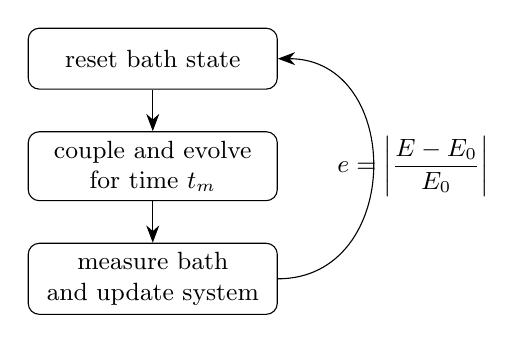
\begin{tikzpicture}[node distance=1.5em and 2.2em, font=\small]
    \tikzstyle{box}=[draw, rounded corners, align=center, minimum height=2.2em, minimum width=9.0em]

    \node[box] (reset) {reset bath state};
    \node[box, below=of reset] (evolve) {couple and evolve\\for time $t_m$};
    \node[box, below=of evolve] (measure) {measure bath\\and update system};

    \draw[-{Stealth[length=2.2mm]}] (reset) -- (evolve);
    \draw[-{Stealth[length=2.2mm]}] (evolve) -- (measure);
    \draw[-{Stealth[length=2.2mm]}] (measure.east) .. controls +(1.6,0) and +(1.6,0) .. (reset.east);

    \node[align=left, right=1.8em of evolve] (metric) {$e = \left|\dfrac{E-E_0}{E_0}\right|$};
  \end{tikzpicture}

  \column{0.45\textwidth}
  \vspace{0.4em}
  \small
  \begin{tabular}{@{}ll@{}}
    \toprule
    object & implementation \\
    \midrule
    backend & ED; TN (MPS/MPO) \\
    state & density matrix; MCWF \\
    evolution & continuous; Trotter \\
    \bottomrule
  \end{tabular}
\end{columns}
\end{frame}

\section{Consistency checks}

\begin{frame}{Consistency check: MCWF vs density matrix (ED)}
  \centering
  \includegraphics[width=0.92\linewidth]{consistency_mcwf_vs_dm_ed.pdf}
\end{frame}

\begin{frame}{Consistency check: TN vs ED (density matrix, Trotter)}
  \centering
  \includegraphics[width=0.95\linewidth]{consistency_tn_vs_ed_dm_trotter.pdf}
\end{frame}

\begin{frame}{K-space notation used in diagnostics}
\small
For periodic or antiperiodic integrable Ising chains, the diagnostics follow
\texttt{Notes/NotesED/MapToSpin.tex}.

\begin{align*}
  \tilde n_k
  &= \langle \tilde a_k^\dagger \tilde a_k\rangle
   = \frac{1}{N}\sum_{m,n} e^{i(m-n)\phi_k}
     \langle a_m^\dagger a_n\rangle,\\
  n_k^{\mathrm{Bog}}
  &= \langle \hat n_k\rangle
   = \frac{1+\langle h_k\rangle}{2},
  \qquad h_k=2\hat a_k^\dagger\hat a_k-1.
\end{align*}

The energy diagnostic is reconstructed from the mode observables,
\begin{equation*}
  E_{\mathrm{modes}}
  =\frac{\Lambda}{2}\sum_{k\in\mathrm{grid}(g_F)}
    \operatorname{coeff}_k\,\langle h_k\rangle,
\end{equation*}
with signed special-mode coefficients.  Thus \(\tilde n_k\) is a raw
Fourier occupation, while \(n_k^{\mathrm{Bog}}\) is a quasiparticle
occupation; neither is an unspecified mode-energy contribution.
\end{frame}

\begin{frame}{Consistency check: mode-resolved reconstruction (Ising, PBC)}
  \centering
  \includegraphics[width=0.95\linewidth]{mode_energy_consistency_ed.pdf}
\end{frame}

\section{Multi-frequency detunings}

\begin{frame}{Multi-frequency detunings (ED, Ising)}
  \centering
  \includegraphics[width=0.95\linewidth]{ground_state_cooling_ising_ed_dm_ZZ_t24_g0.02_R15.pdf}
\end{frame}

\begin{frame}{Multi-frequency detunings (TN, Ising $N=20$)}
  \centering
  \includegraphics[width=0.95\linewidth]{ground_state_cooling_ising_tn_mcwf_trotter_ZZ_N20_g0.2_te3.2_steps80_R15.pdf}
\end{frame}

\section{Randomized cycle times}

\begin{frame}{Randomized cycle times (ED, MCWF)}
  \centering
  \includegraphics[width=0.95\linewidth]{randomized_times_remove_accidental_heating_ed_ising_mcwf_multiR15_relative.pdf}
\end{frame}

\section{Summary}

\begin{frame}{Summary}
\small
\begin{itemize}
  \item ED/TN and DM/MCWF comparisons provide consistency checks in regimes where both are available.
  \item Multi-frequency detunings improve cooling performance compared to single-$\Delta$ protocols (ED and TN examples).
  \item Randomizing the cycle time suppresses accidental resonances in a scan over mean evolution times (ED example).
\end{itemize}

\vspace{0.8em}
\small
Next: apply the same analysis to the non-integrable Ising model; extend TN runs to larger $N$ and perform parameter/convergence scans.
\end{frame}

\end{document}
